%===========================================
%  Acceptance
%===========================================

\section{ Acceptance }
\slide{ Quick look at acceptance }
{
Effect of generators, $\Wboson$ $p_T$ and PDF reweighting on acceptance
\centering
\only<1>{\footnotesize{Total acceptance }}
\only<2>{\footnotesize{Acceptance for $p_T>25 \GeV$ (vs $p_T>20 \GeV$) }}
\colb[T]
\column{.5\textwidth}
\centering
Muon $\Wminus$ acceptance \\
\includegraphics[width=1.0\textwidth]<1>{dates/20121119/figures/acceptance/acceptance_NEG_total.pdf}
\includegraphics[width=1.0\textwidth]<2>{dates/20121119/figures/acceptance/acceptance_NEG_25GeV.pdf}

\column{.5\textwidth}
\centering
Muon $\Wplus$ acceptance \\
\includegraphics[width=1.0\textwidth]<1>{dates/20121119/figures/acceptance/acceptance_POS_total.pdf}
\includegraphics[width=1.0\textwidth]<2>{dates/20121119/figures/acceptance/acceptance_POS_25GeV.pdf}
\cole

}

%===========================================
%  Systematics
%===========================================

\section{ Systematics }
\slide{ Corrected systematic uncertainties }
{
\centering
A script Max and I were using to plot uncertainties had a bug \\
(Systematics where the histogram drops below Nominal weren't shown)
\colb[T]
\column{.5\textwidth}
\centering
Muon $\Wminus$ uncertainties \\
\includegraphics[width=1.0\textwidth]<1>{dates/20121119/figures/unfold/old_1d_NEG.pdf}
\includegraphics[width=1.0\textwidth]<2>{dates/20121119/figures/unfold/new_1d_NEG.pdf}

\column{.5\textwidth}
\centering
Muon $\Wplus$ uncertainties \\
\includegraphics[width=1.0\textwidth]<1>{dates/20121119/figures/unfold/old_1d_POS.pdf}
\includegraphics[width=1.0\textwidth]<2>{dates/20121119/figures/unfold/new_1d_POS.pdf}
\cole

\only<1>{\footnotesize{Some systematics are hidden under the 0\% line }}
\only<2>{\footnotesize{All systematics are present because $|abs|$ was added }}
}

%===========================================
%  Systematics (2D)
%===========================================

\slide{2D systematics: $\Wplus \rightarrow \mu^+ \nu$}
{
  \centering
  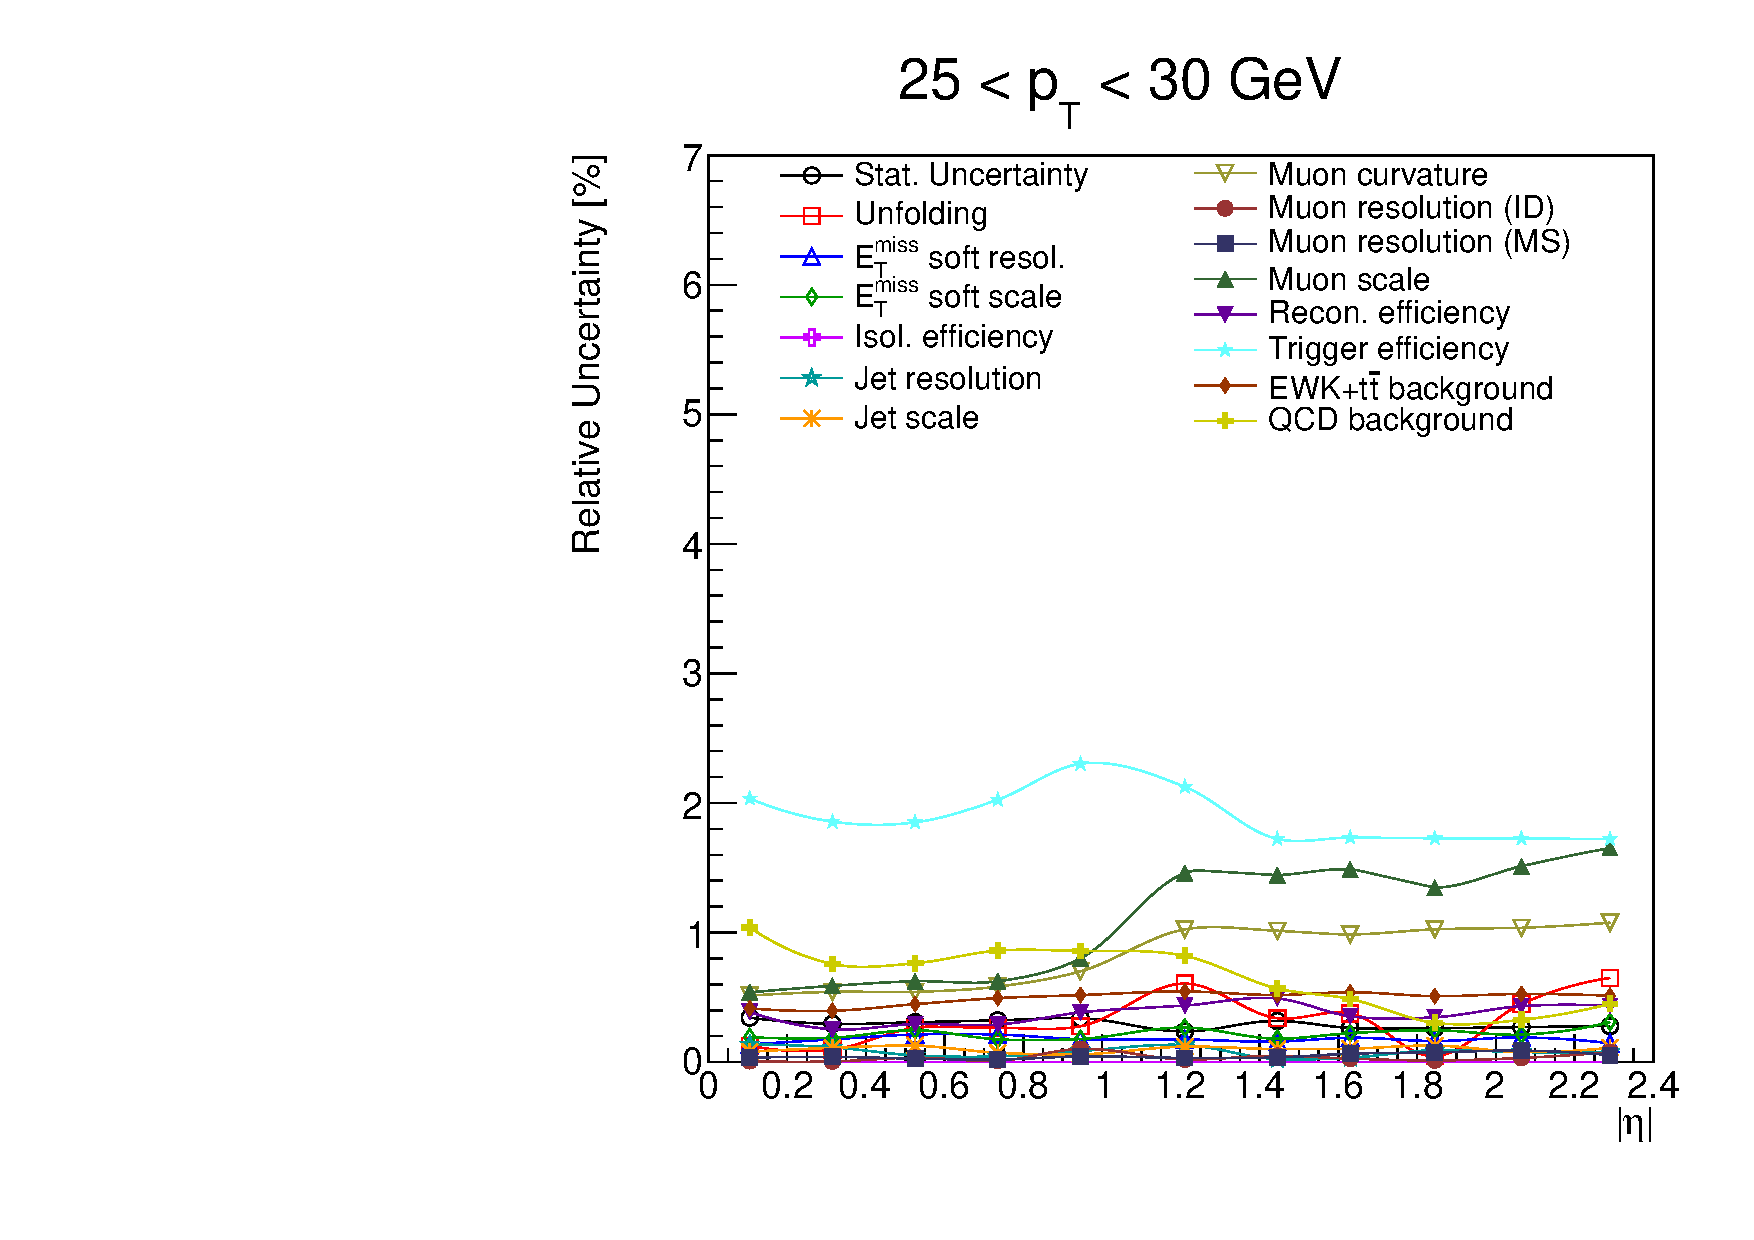
\includegraphics[width=0.3\textwidth]{dates/20121119/figures/unfold/uncertainties_pos_2.pdf}
  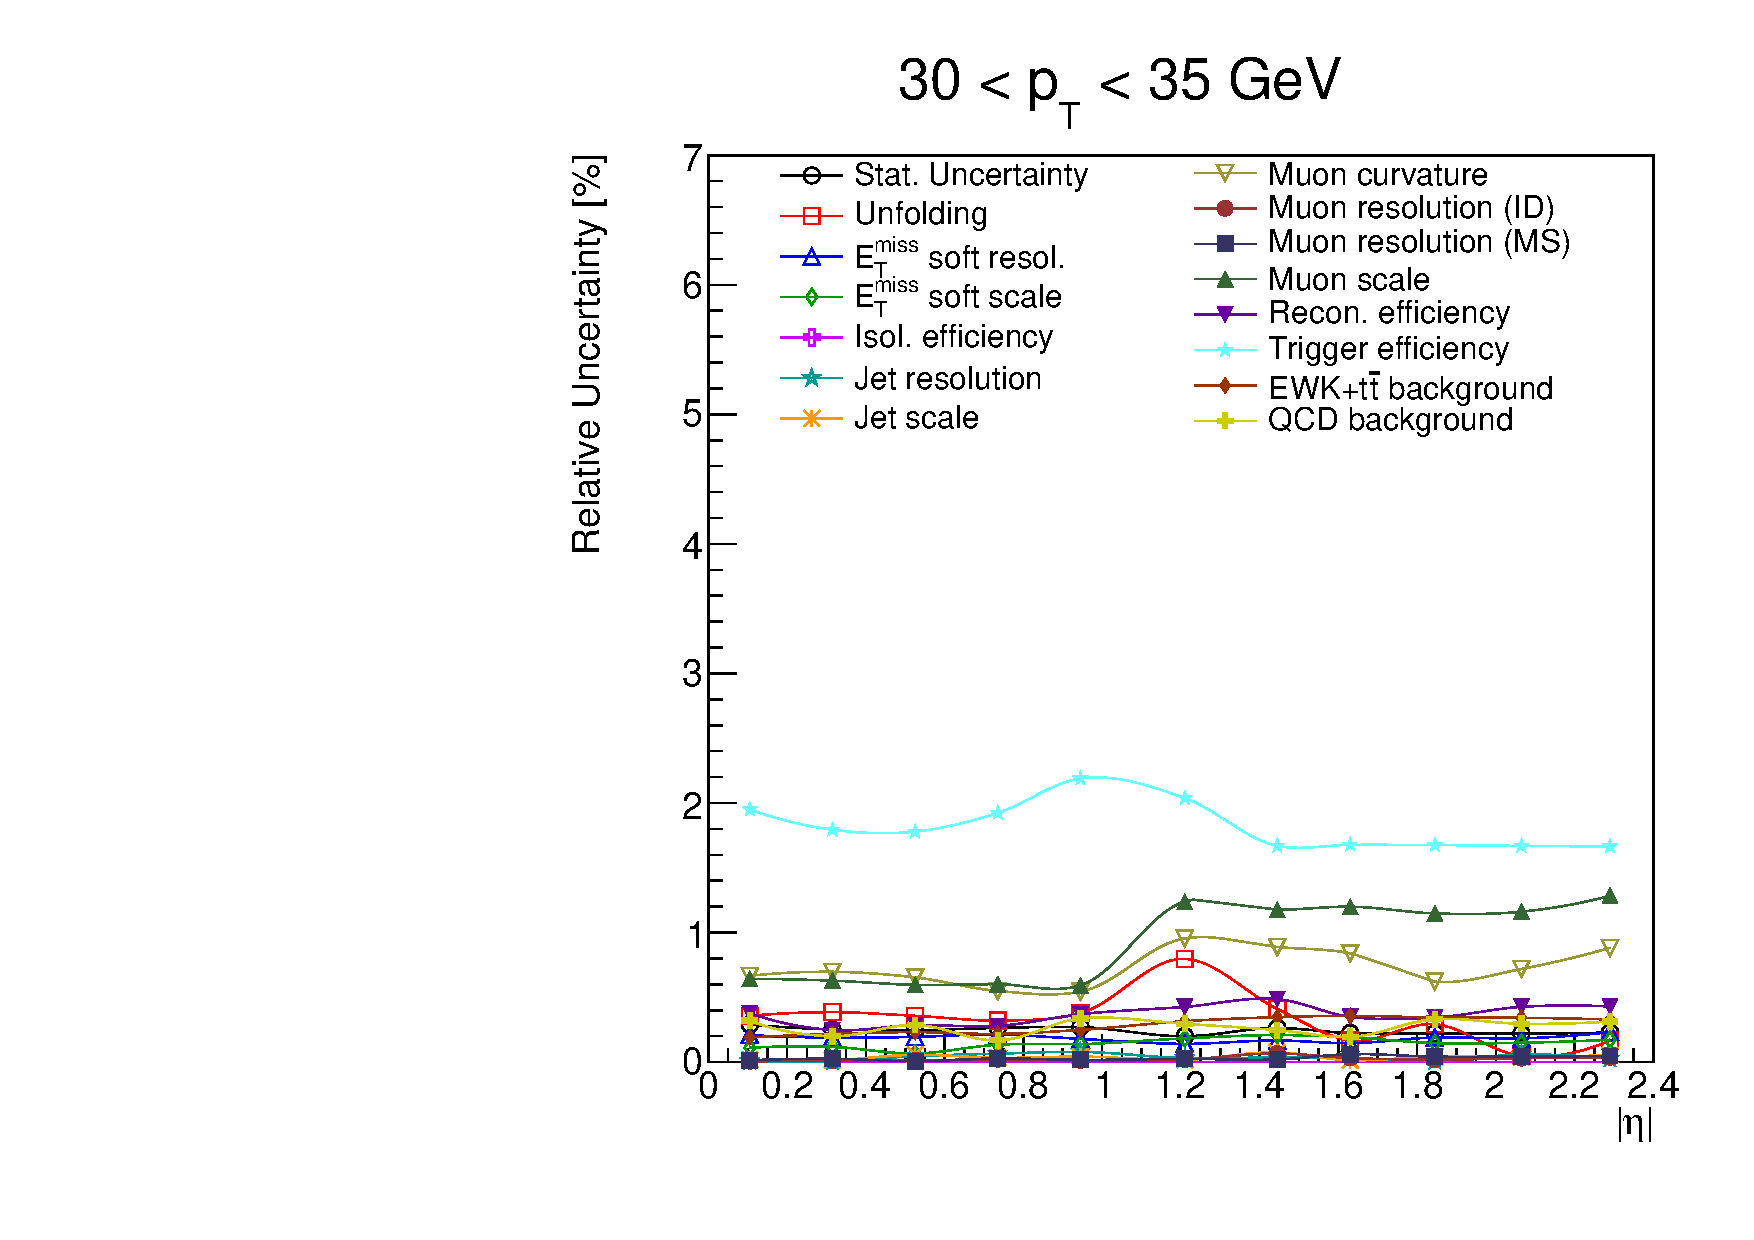
\includegraphics[width=0.3\textwidth]{dates/20121119/figures/unfold/uncertainties_pos_3.pdf}
  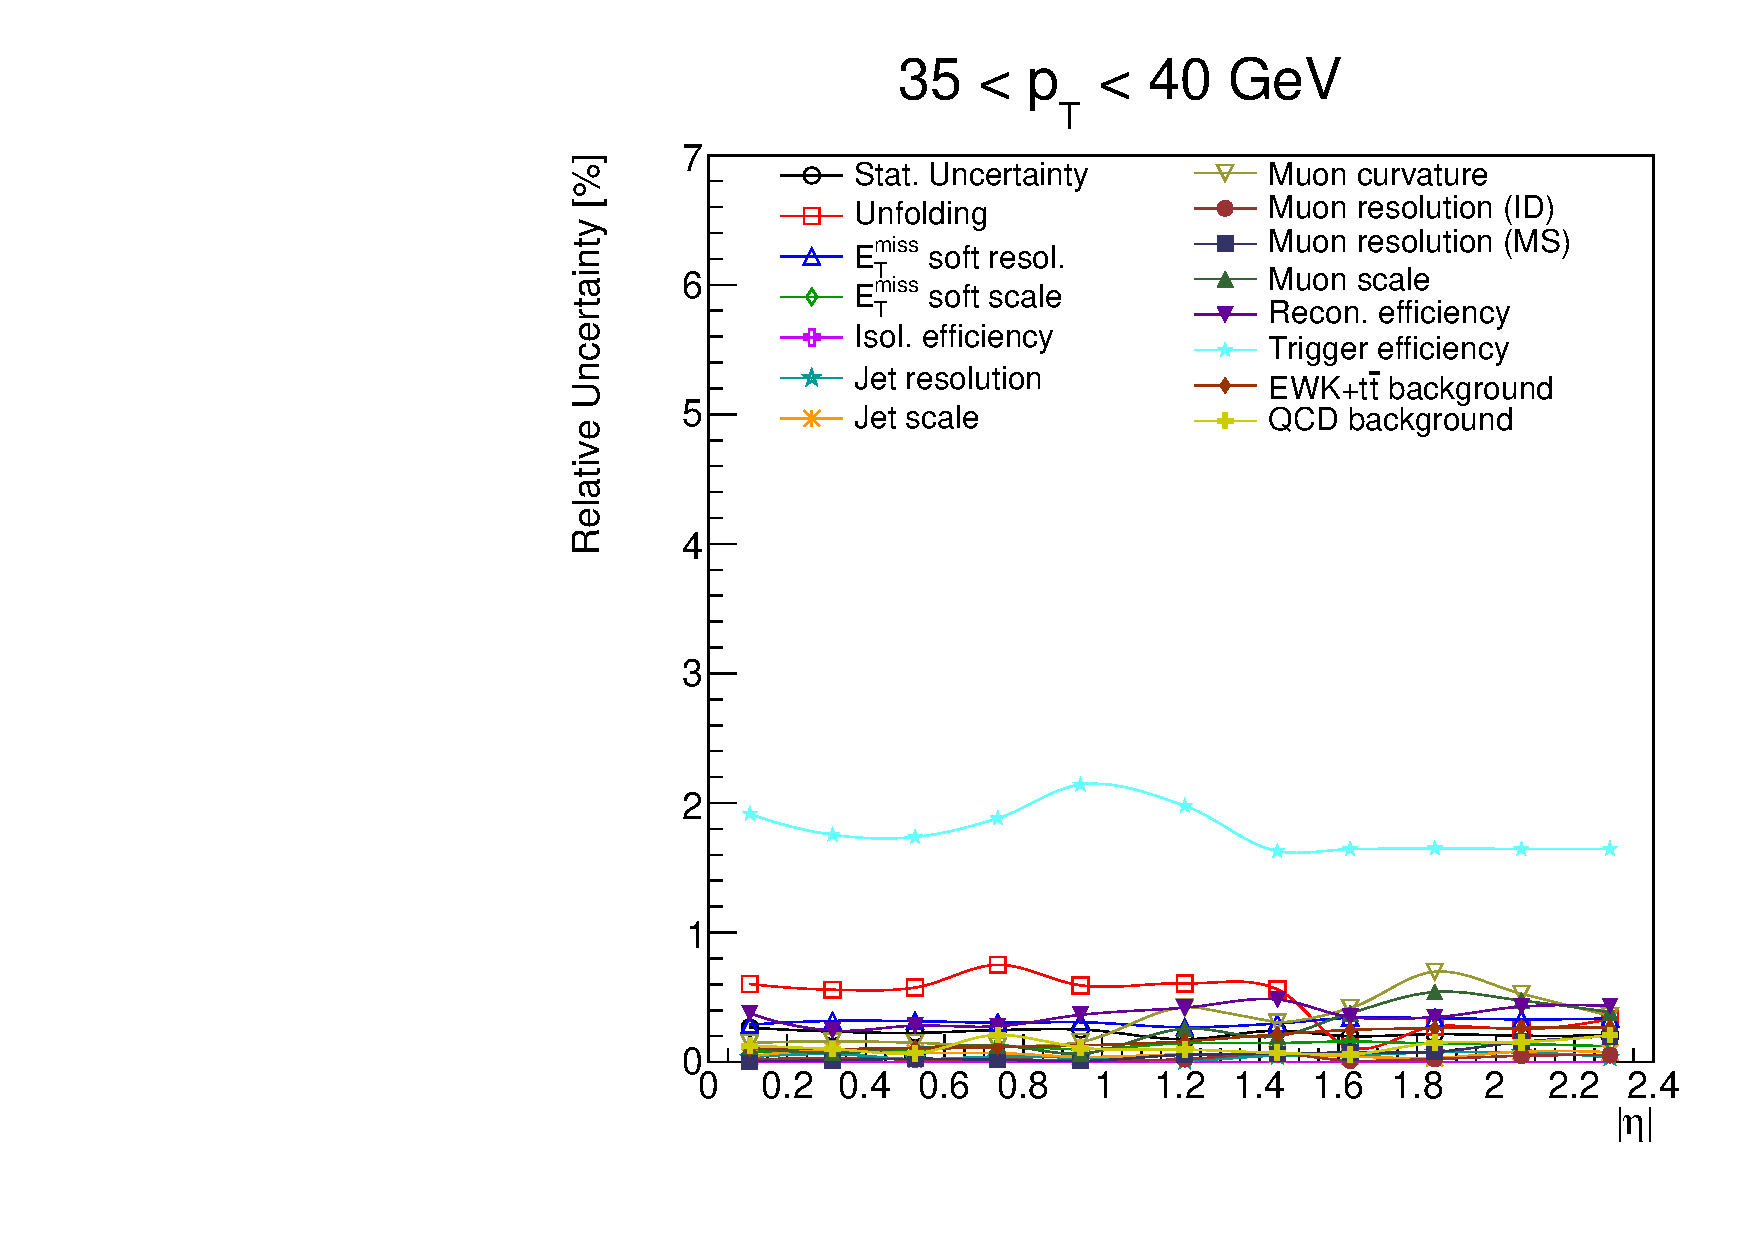
\includegraphics[width=0.3\textwidth]{dates/20121119/figures/unfold/uncertainties_pos_4.pdf}
  \newline
  \centering
  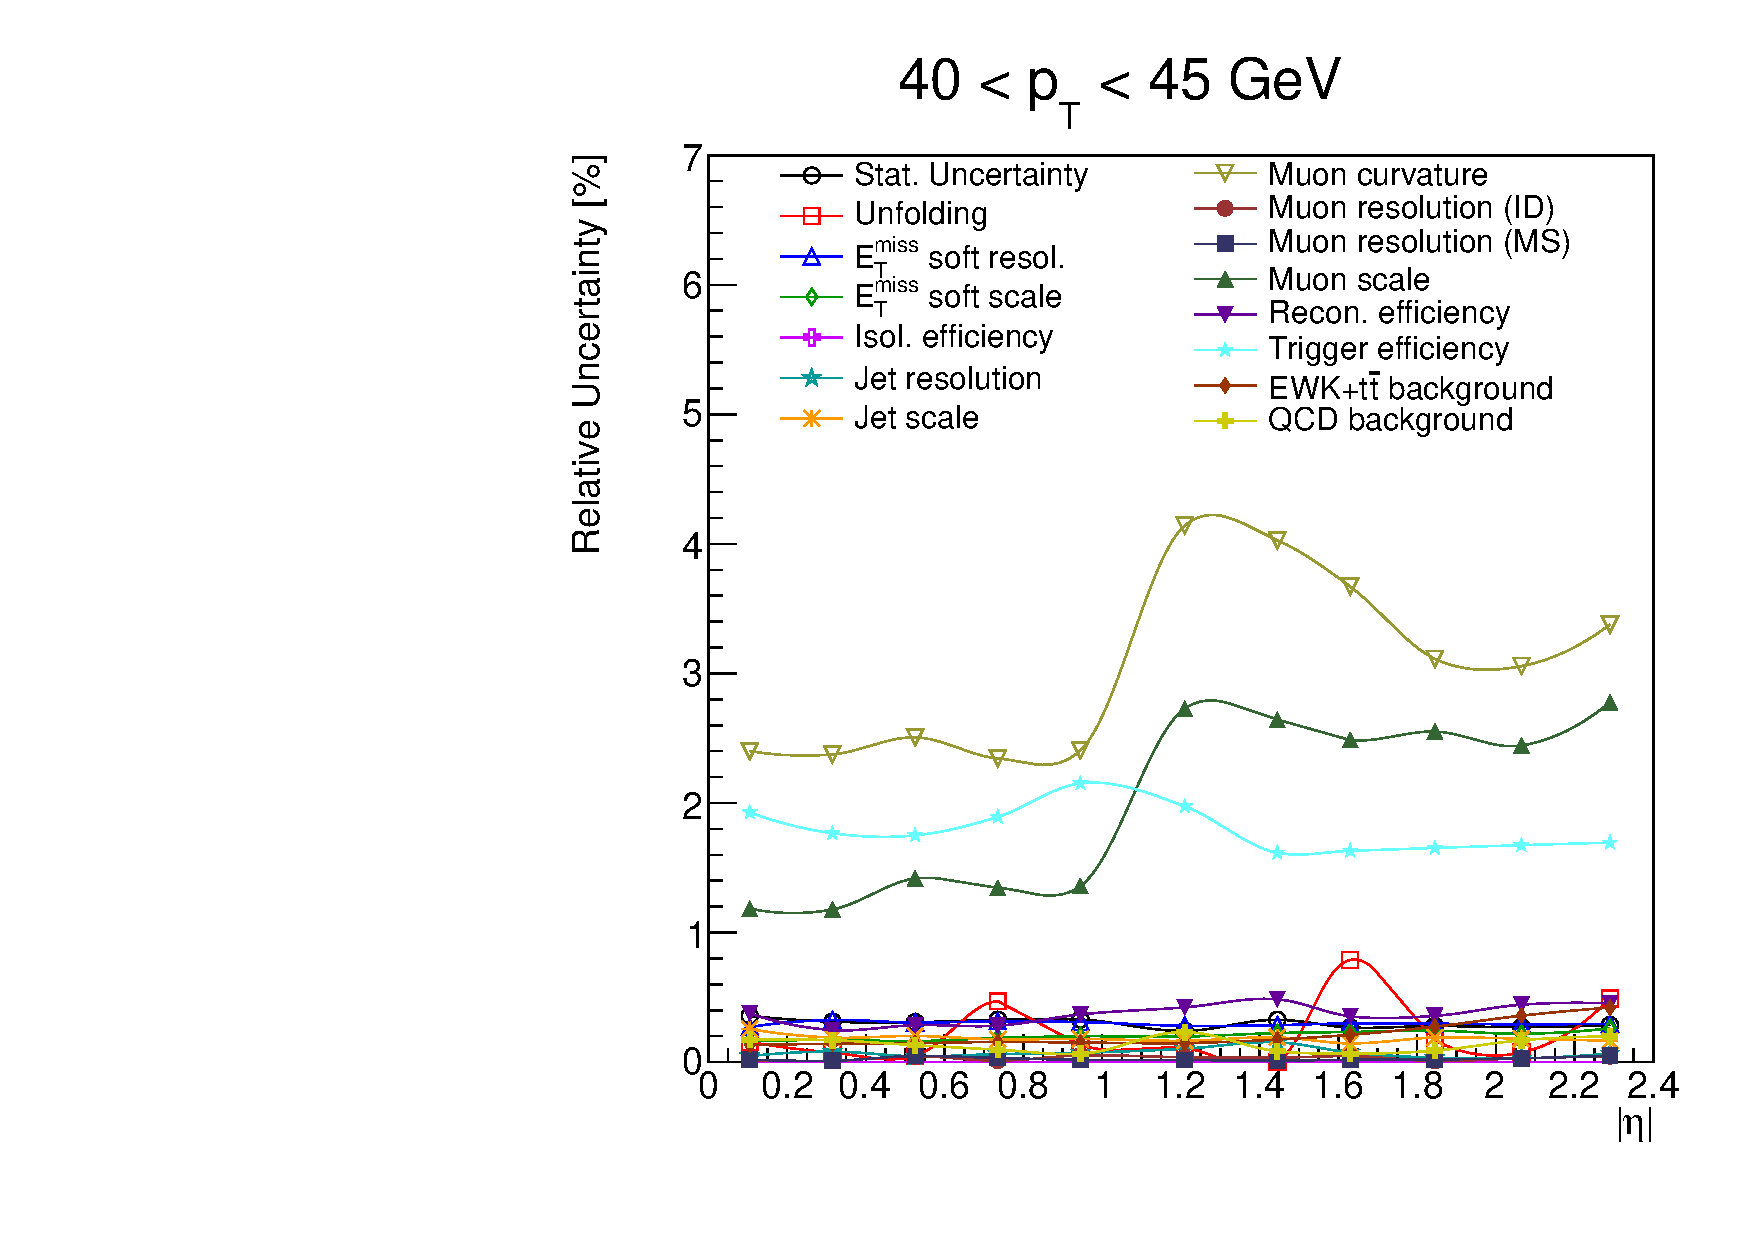
\includegraphics[width=0.3\textwidth]{dates/20121119/figures/unfold/uncertainties_pos_5.pdf}
  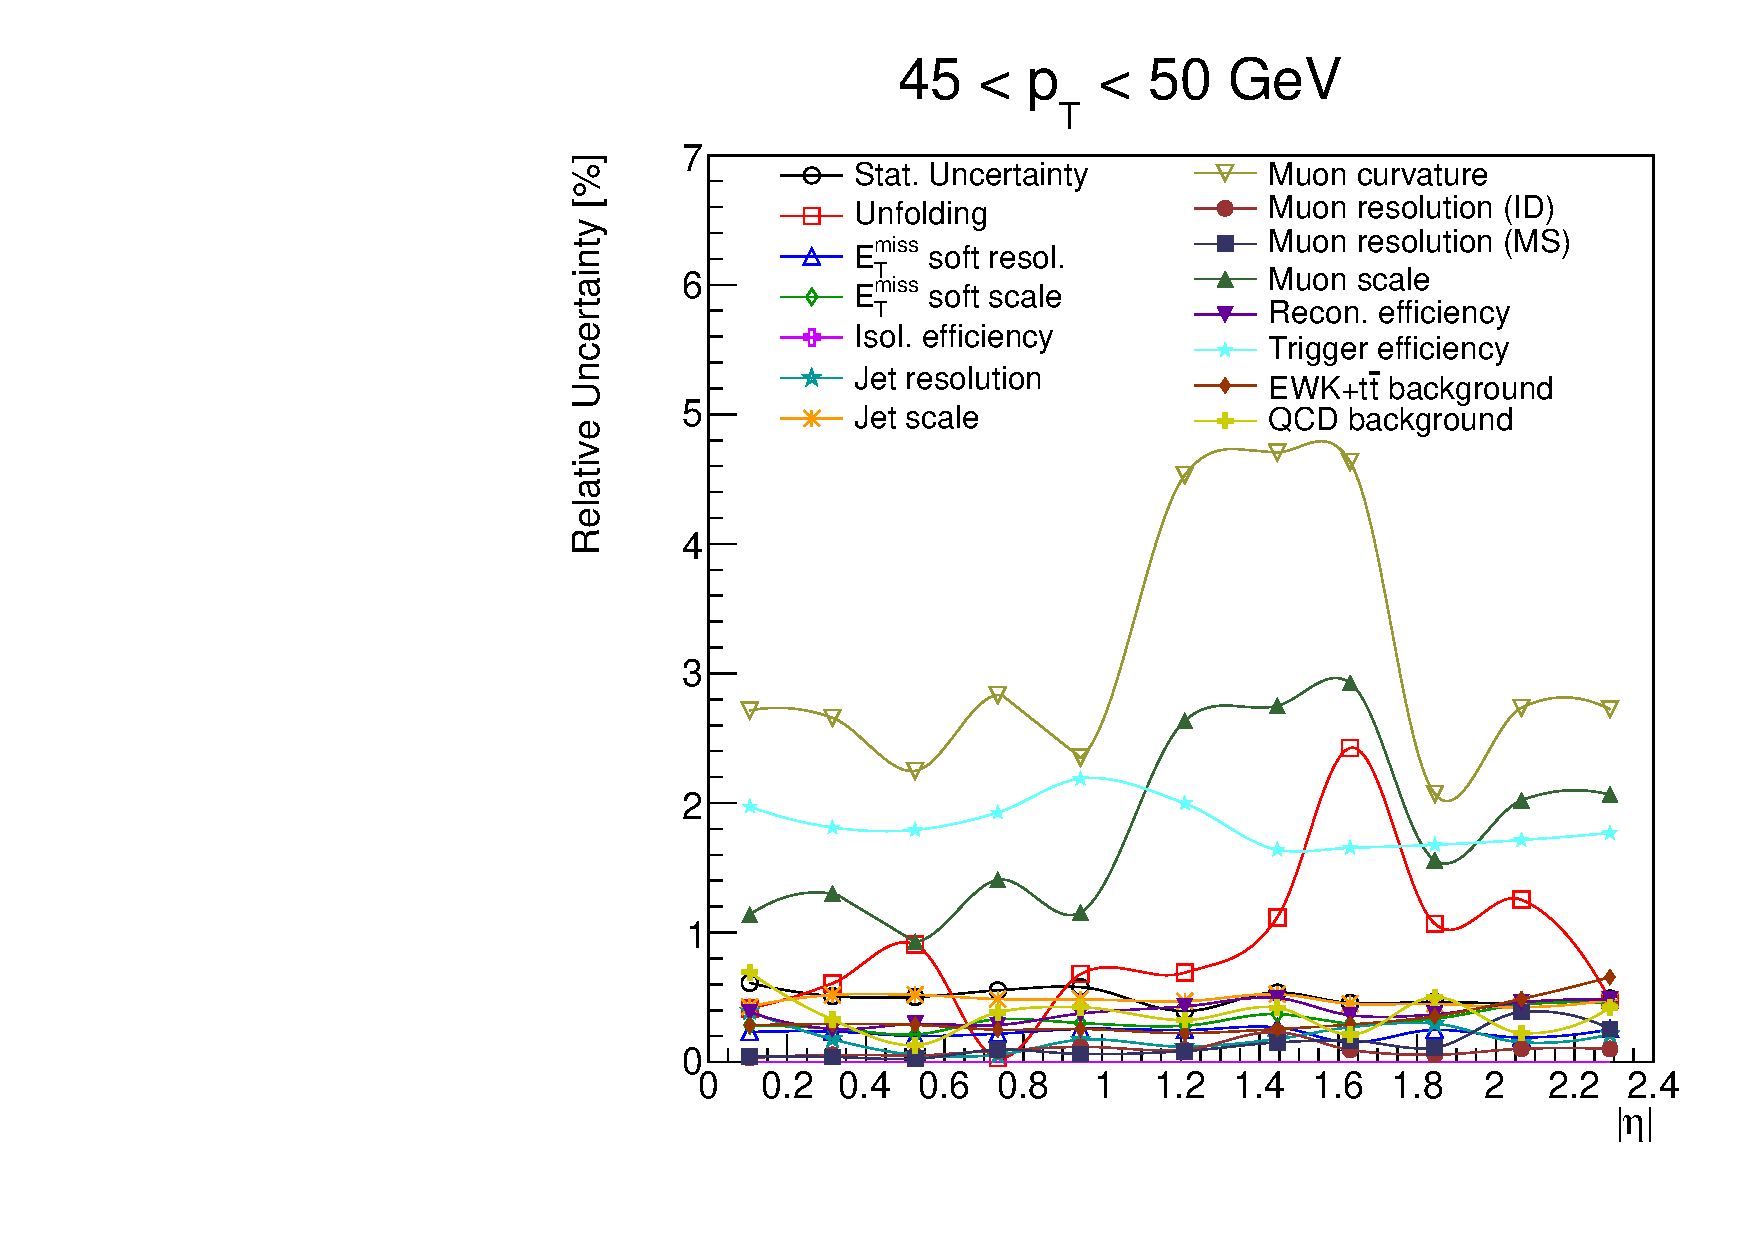
\includegraphics[width=0.3\textwidth]{dates/20121119/figures/unfold/uncertainties_pos_6.pdf}
  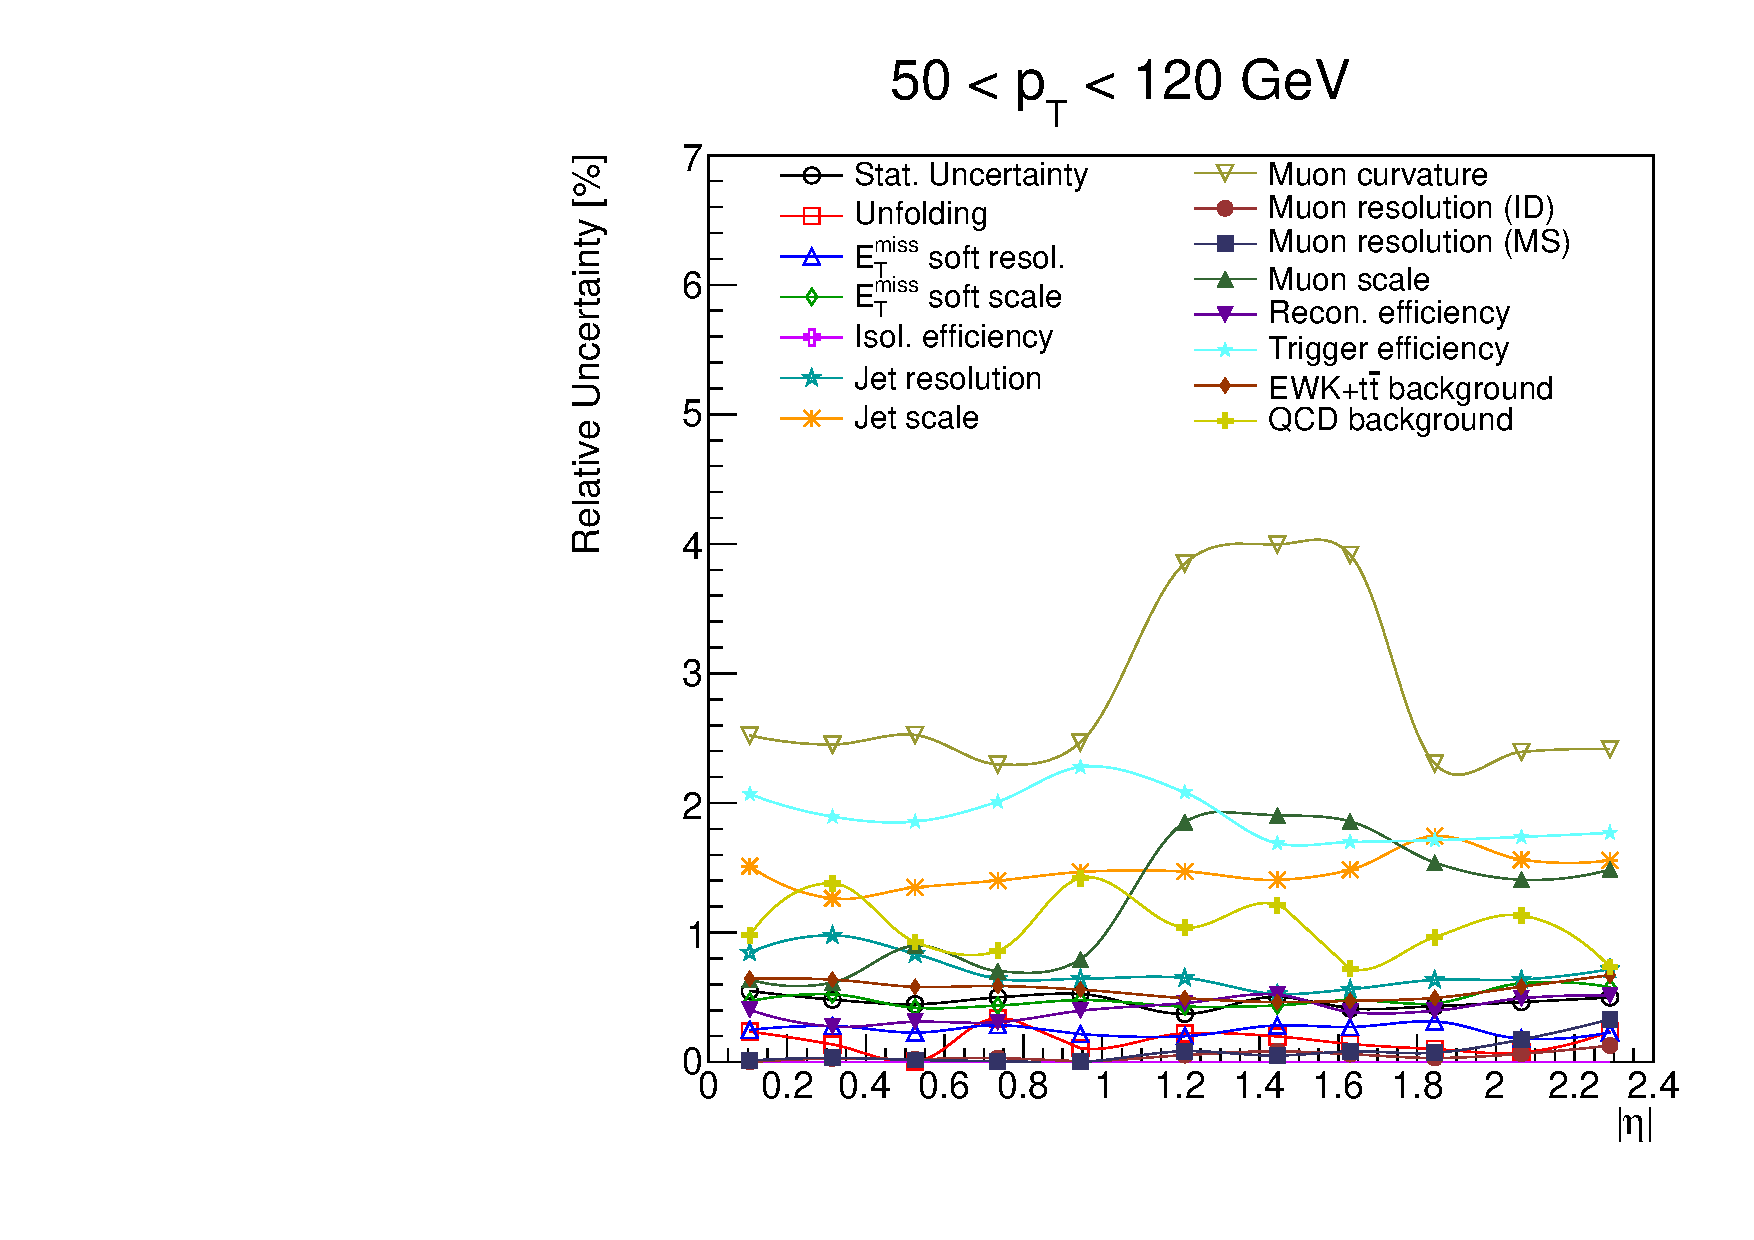
\includegraphics[width=0.3\textwidth]{dates/20121119/figures/unfold/uncertainties_pos_7.pdf}
  \newline
  \footnotesize{Notice how previously unseen \red{muon momentum systematics dominate}.}
}

\slide{2D systematics: $\Wminus \rightarrow \mu^- \nu$}
{
  \centering
  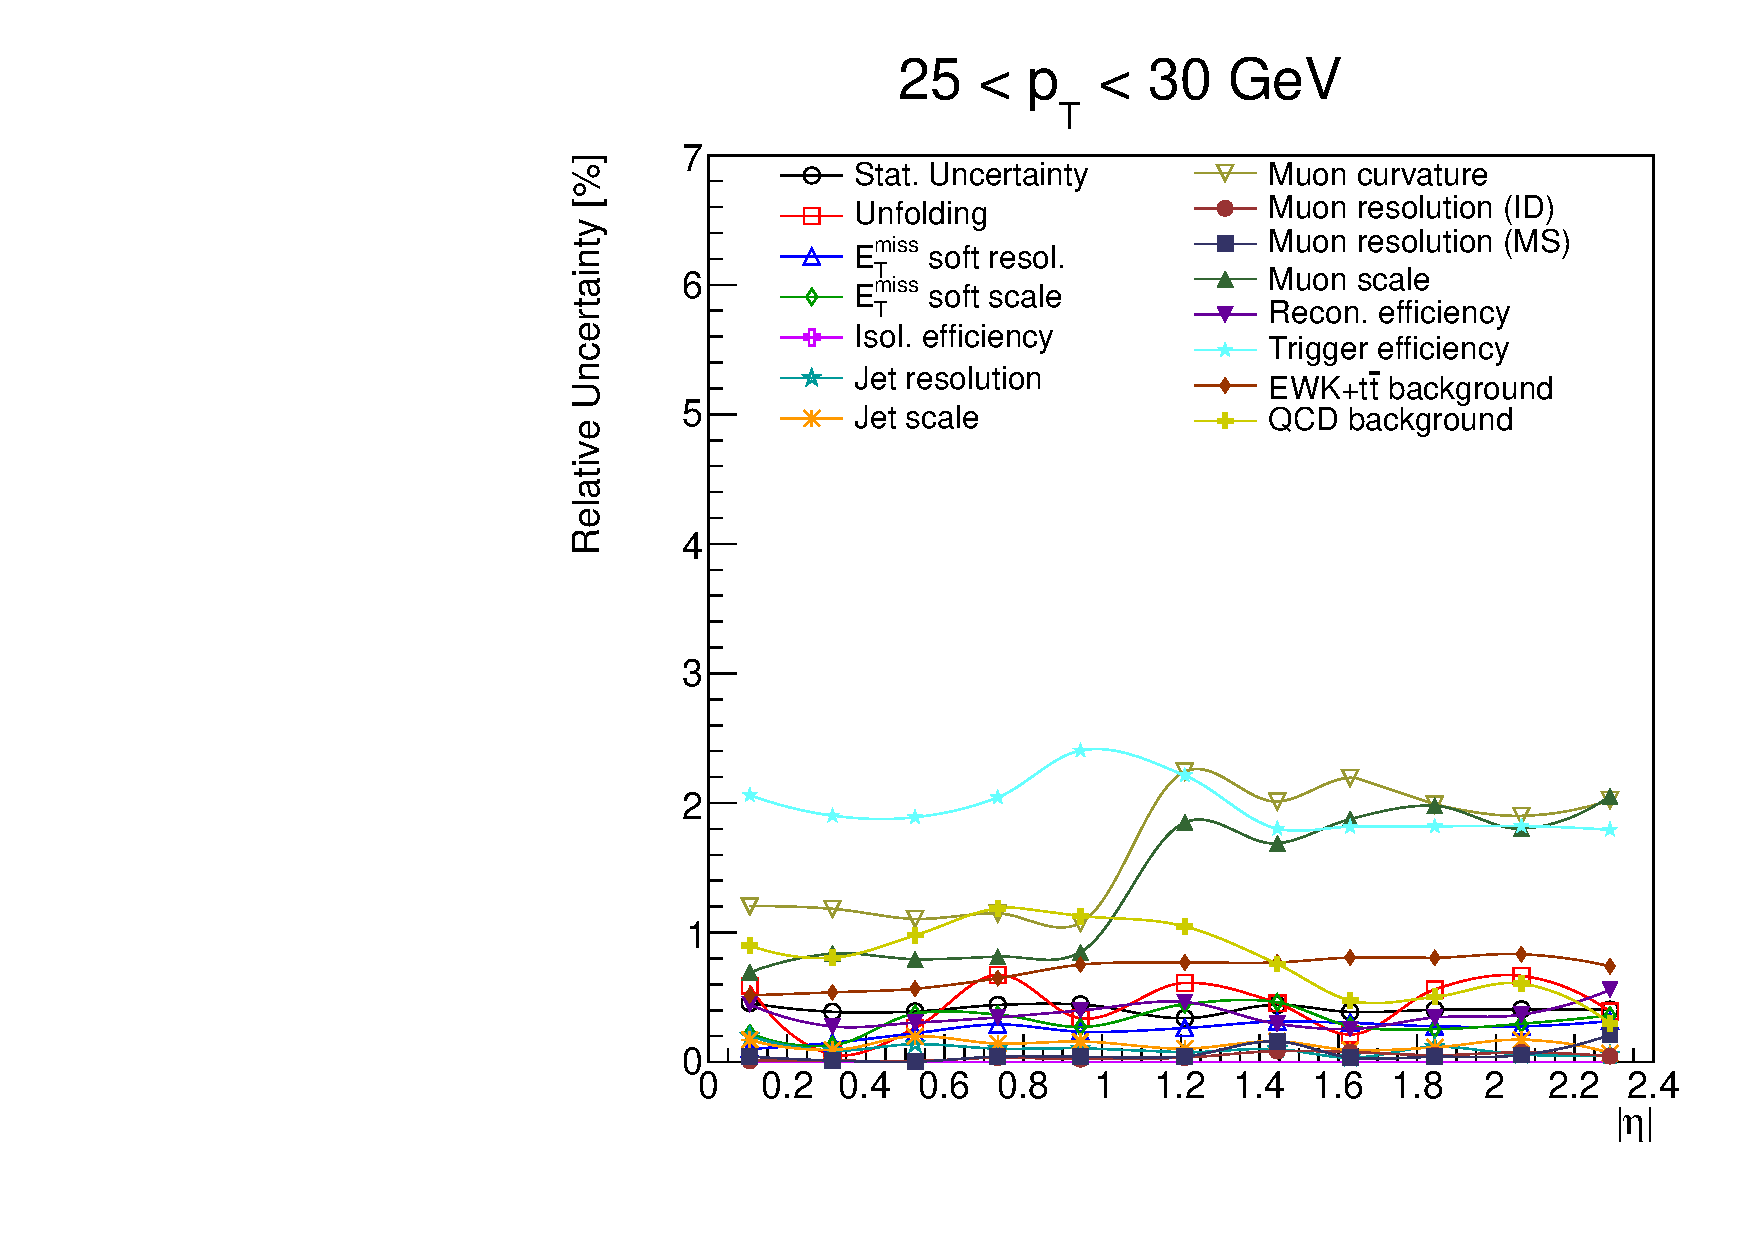
\includegraphics[width=0.3\textwidth]{dates/20121119/figures/unfold/uncertainties_neg_2.pdf}
  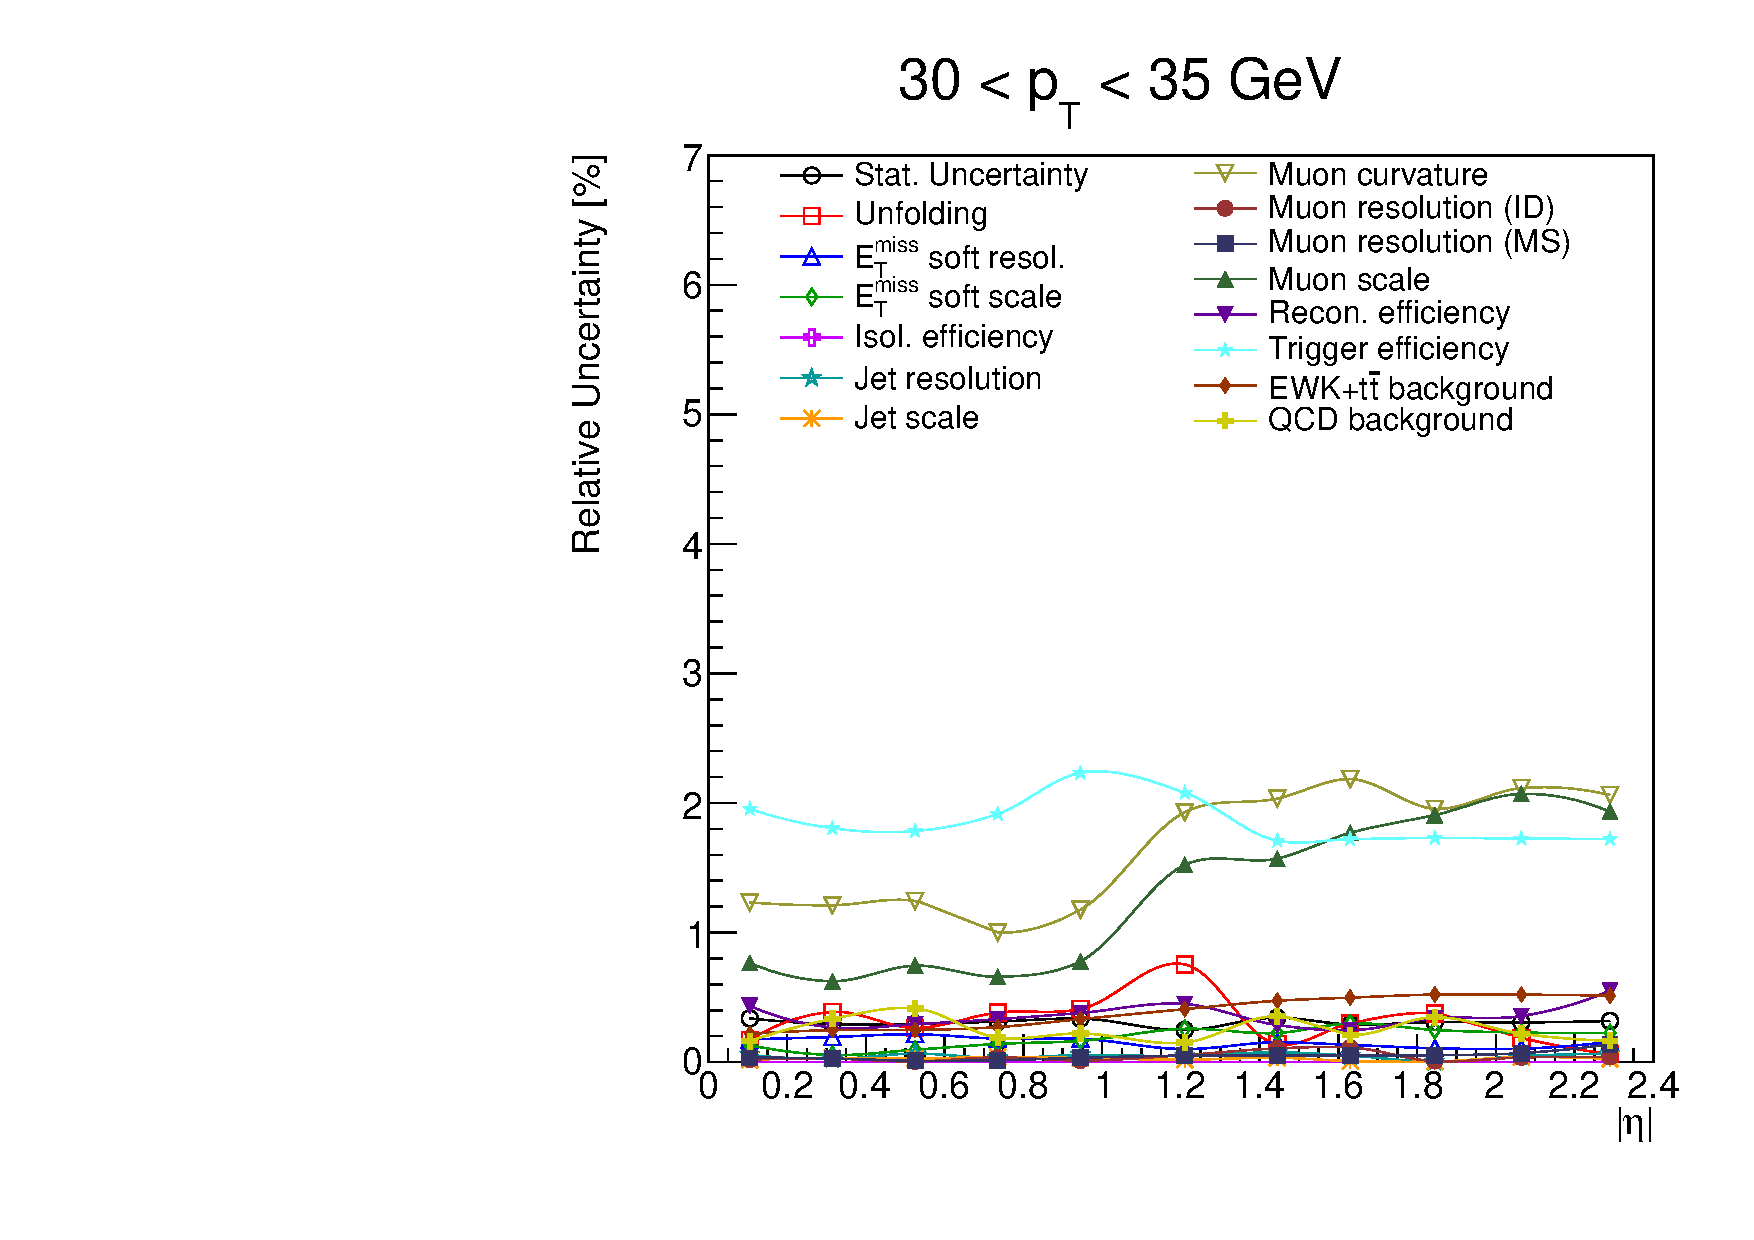
\includegraphics[width=0.3\textwidth]{dates/20121119/figures/unfold/uncertainties_neg_3.pdf}
  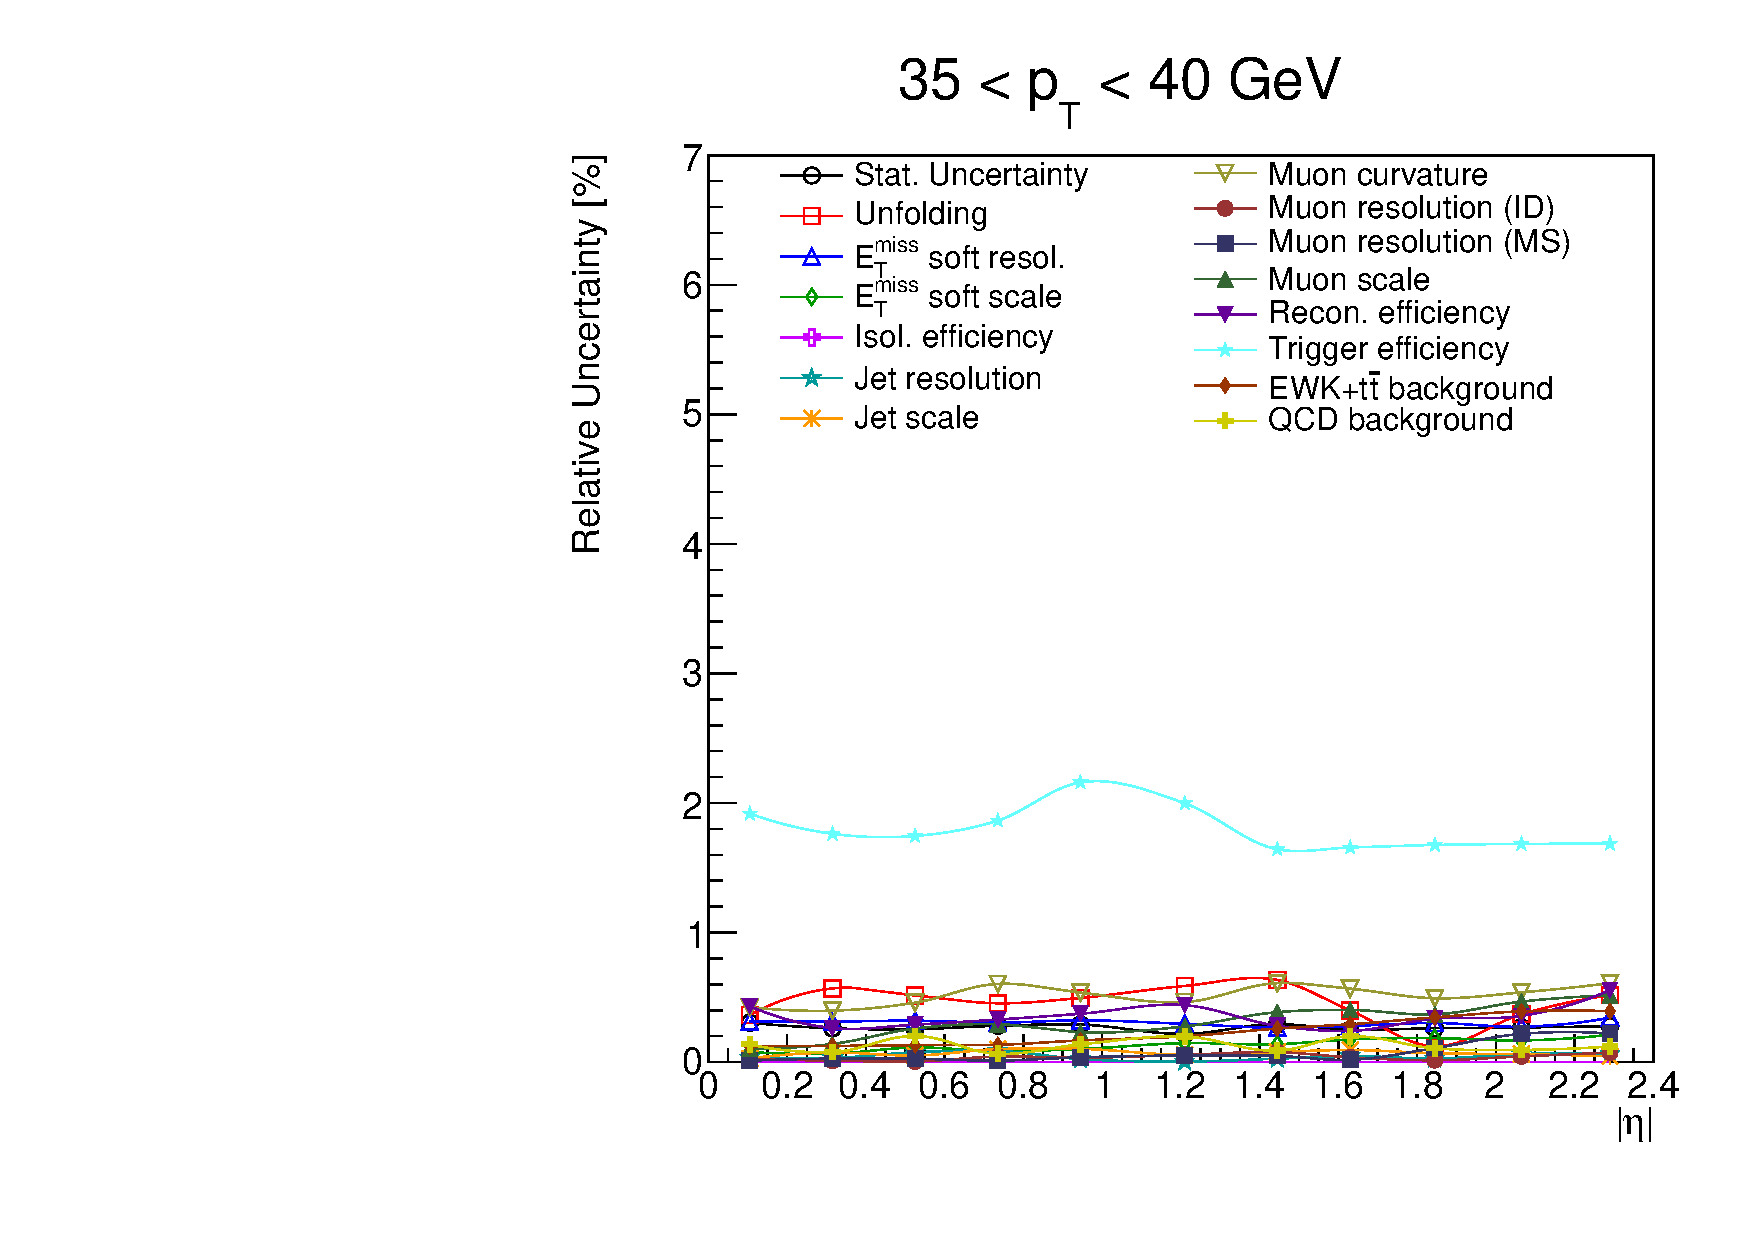
\includegraphics[width=0.3\textwidth]{dates/20121119/figures/unfold/uncertainties_neg_4.pdf}
  \newline
  \centering
  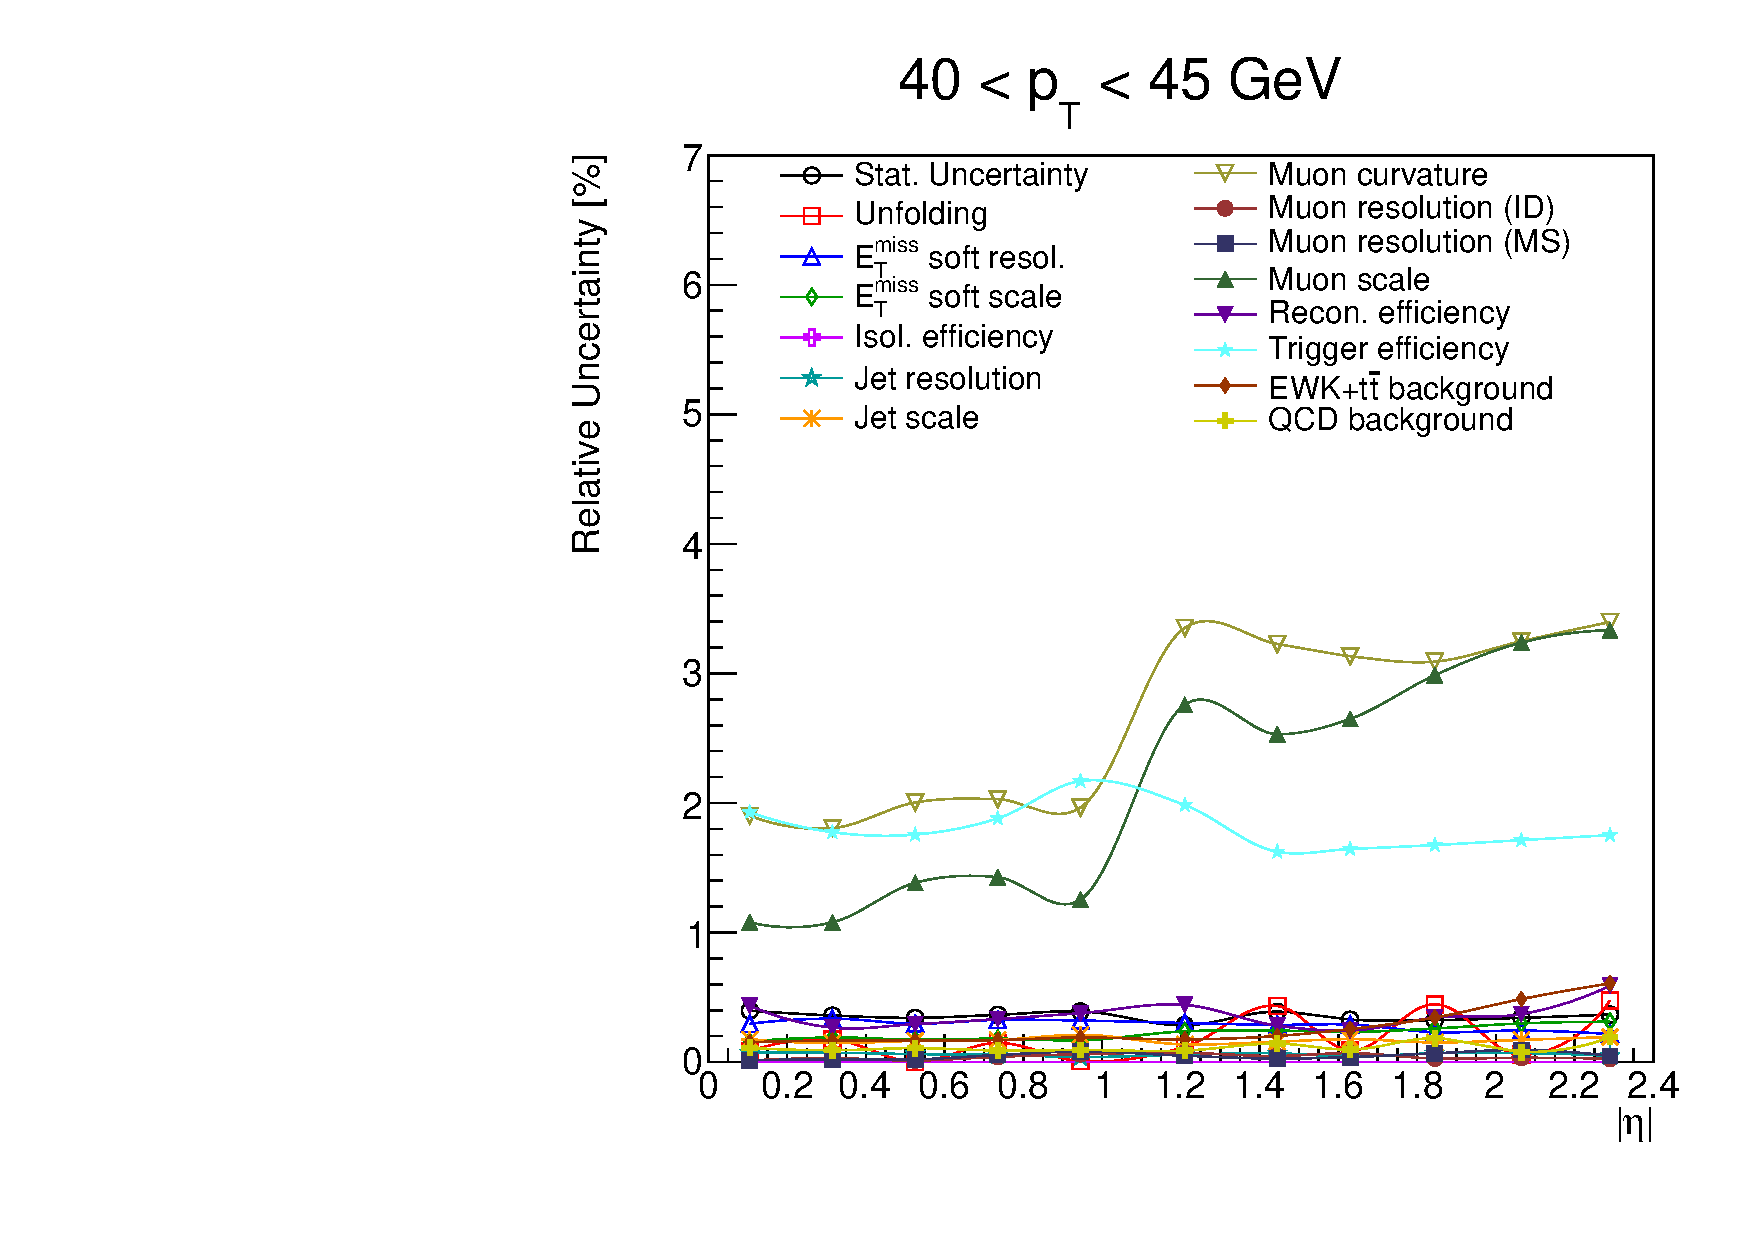
\includegraphics[width=0.3\textwidth]{dates/20121119/figures/unfold/uncertainties_neg_5.pdf}
  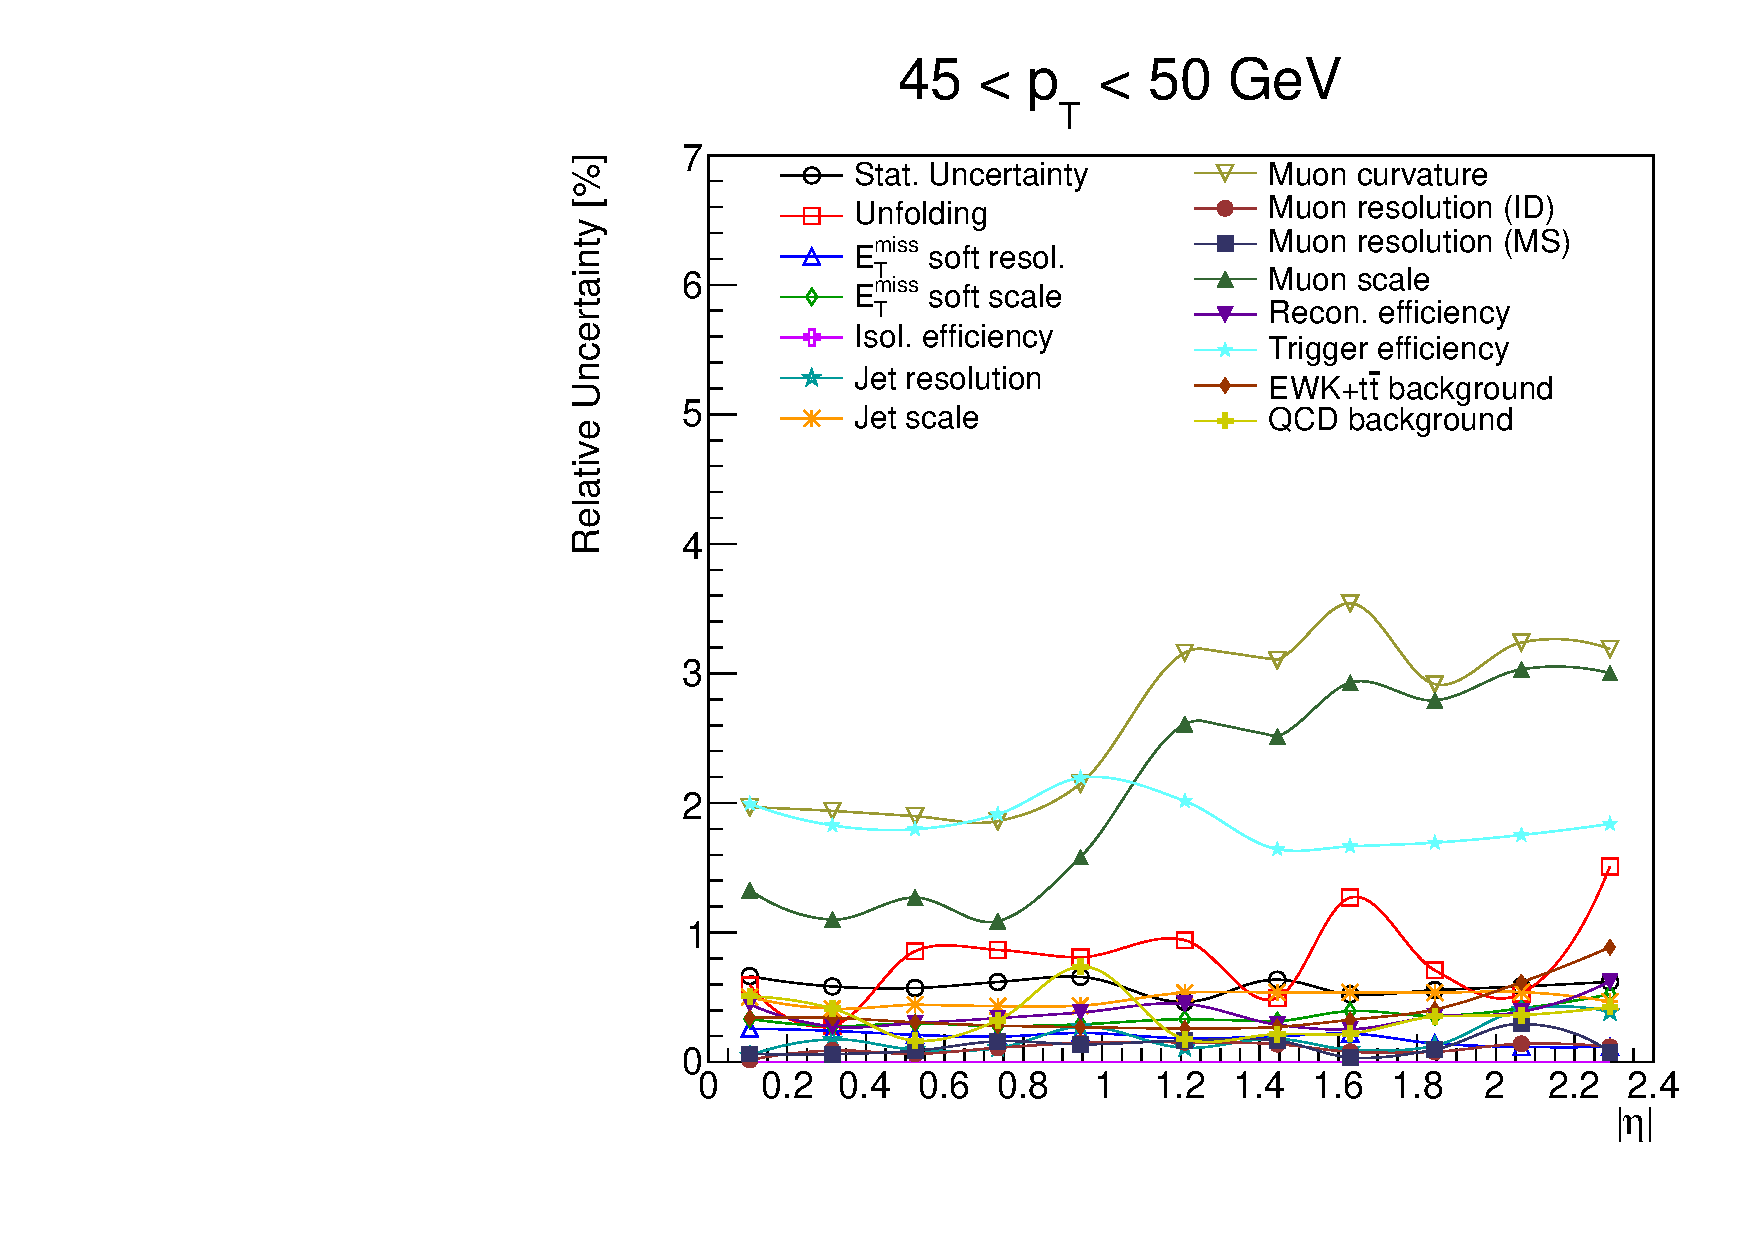
\includegraphics[width=0.3\textwidth]{dates/20121119/figures/unfold/uncertainties_neg_6.pdf}
  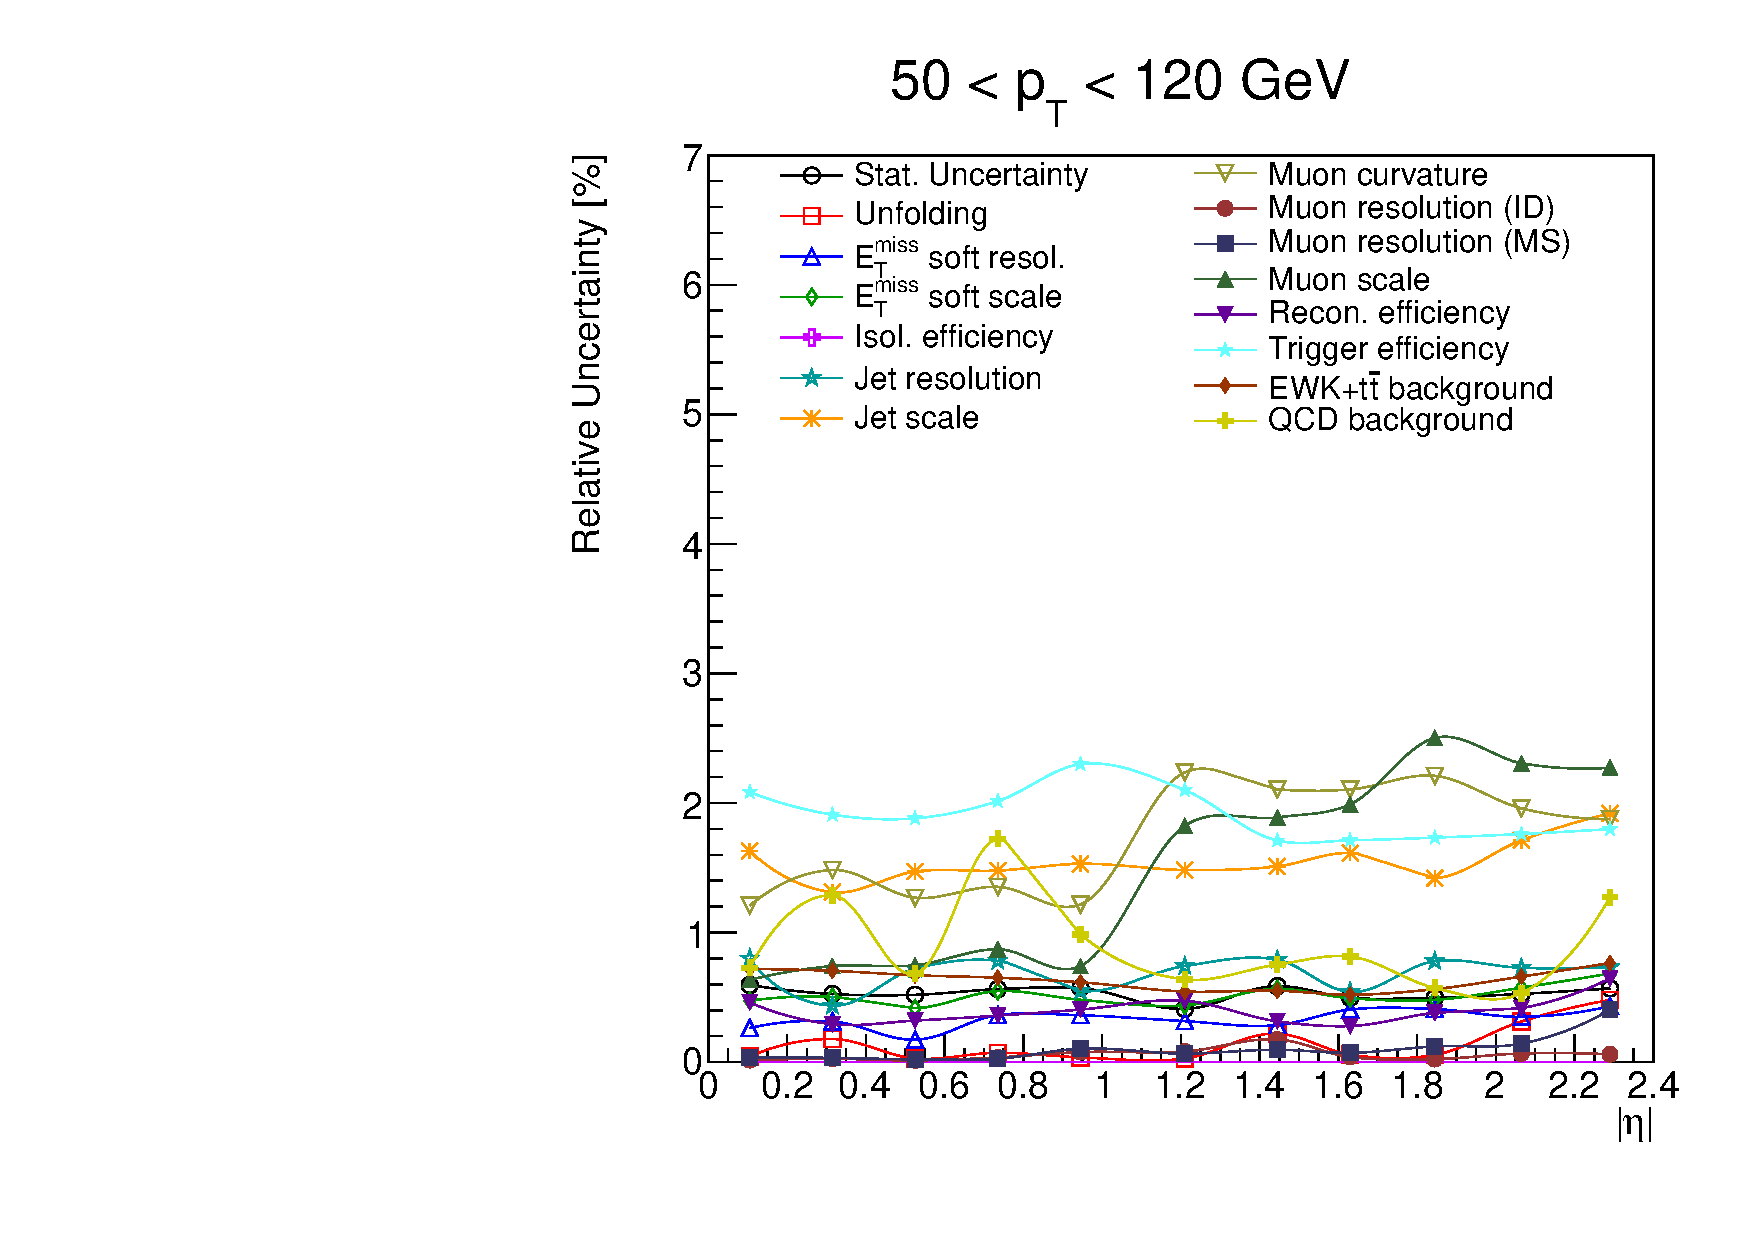
\includegraphics[width=0.3\textwidth]{dates/20121119/figures/unfold/uncertainties_neg_7.pdf}
  \newline
  \footnotesize{Notice how previously unseen \red{muon momentum systematics dominate}.}
}


\slide{ Comment on muon momentum systematics }
{
  One caveat in the above plots is that the response matrices were produced with an outdated version of MuonMomentumCorrections, where muon momentum scale and curvature systematics are (incorrectly) applied ``twice-over''. So we need to check how these plots look with the fixed version.
}
%===========================================
%  Asymmetry and uncertainties
%===========================================

\section{ Asymmetry }
\slide{ Systematics on asymmetry }
{
\centering
$\Wboson$ charge asymmetry \\
\includegraphics[width=0.6\textwidth]<1>{dates/20121119/figures/asym/Wmn_Unf_proj.pdf}
\includegraphics[width=0.6\textwidth]<2>{dates/20121119/figures/asym/Wmn_unf2010_proj.pdf}
\includegraphics[width=0.6\textwidth]<3>{dates/20121119/figures/asym/Wmn_Unc2_proj.pdf}

\only<1>{\footnotesize{Compared to Powheg+Pythia }}
\only<2>{\footnotesize{Compared to 2010 }}
\only<3>{\footnotesize{Systematics (dominated by charge-splitting muon curvature, as expected) }}

}

%===========================================
%  Studying new trigger scale factors
%===========================================

\section{ Trigger corrections }

\slide{Effect of new $\eta-\phi$ muon trigger corrections}
{
\centering
\alt<1,3>{\purple{Old} corrections in $\eta-p_{T}$ only}{\purple{New} corrections in $\eta-p_{T}$ x $\eta-phi$}

\colb[T]
\column{.5\textwidth}
\centering
Muon $\Wminus$ \alt<1,2>{$eta$}{$phi$} \\
\includegraphics[width=1.0\textwidth]<1>{dates/20121119/figures/trig/old_eta_NEG.pdf}
\includegraphics[width=1.0\textwidth]<2>{dates/20121119/figures/trig/new_eta_NEG.pdf}
\includegraphics[width=1.0\textwidth]<3>{dates/20121119/figures/trig/old_phi_NEG.pdf}
\includegraphics[width=1.0\textwidth]<4>{dates/20121119/figures/trig/new_phi_NEG.pdf}

\column{.5\textwidth}
\centering
Muon $\Wplus$ \alt<1,2>{$eta$}{$phi$} \\
\includegraphics[width=1.0\textwidth]<1>{dates/20121119/figures/trig/old_eta_POS.pdf}
\includegraphics[width=1.0\textwidth]<2>{dates/20121119/figures/trig/new_eta_POS.pdf}
\includegraphics[width=1.0\textwidth]<3>{dates/20121119/figures/trig/old_phi_POS.pdf}
\includegraphics[width=1.0\textwidth]<4>{dates/20121119/figures/trig/new_phi_POS.pdf}
\cole
\only<1>{\footnotesize{Positive-negative $\eta$ appears asymmetric: even ignoring choppiness, A-side seems higher. }}
\only<2>{\footnotesize{No obvious improvement. In fact, the \red{last eta bin} seems to have gotten worse.}}
\only<3>{\footnotesize{A lot of structure in $\phi$. The structure is mostly charge-symmetric. }}
\only<4>{\footnotesize{But adding the new $\phi$ corrections \red{does not seem to make it better}. Bug? }}
}

\slide{Plotting event trigger weights in signal MC }
{
\centering
\alt<1,2>{Old corrections in $\eta-p_{T}$ only}{New corrections in $\eta-p_{T}$ x $\eta-phi$}
\colb[T]
\column{.5\textwidth}
\centering
Muon $\Wminus$ trigger weight \\
\includegraphics[width=0.8\textwidth]<1>{dates/20121119/figures/trig/old_trigw_NEG.pdf}
\includegraphics[width=0.8\textwidth]<2>{dates/20121119/figures/trig/new_trigw_NEG.pdf}

\column{.5\textwidth}
\centering
Muon $\Wplus$ trigger weight \\
\includegraphics[width=0.9\textwidth]<1>{dates/20121119/figures/trig/old_trigw_POS.pdf}
\includegraphics[width=0.9\textwidth]<2>{dates/20121119/figures/trig/new_trigw_POS.pdf}
\cole

\only<1>{\footnotesize{``Choppiness'' is due to binned nature of the trigger scale factors. }}
\only<2>{\footnotesize{Note a higher RMS and more smoothness due to large phase space of corrections.}}
}

%===========================================
%  Studying different definitions of nevets
%===========================================

\section{ Nevents and weights }

\slide{Choosing different sum of weights for nevents}
{
\centering
\only<1>{ weight = mc (always 1.0, except for MC@NLO) }
\only<2>{ weight = mc x pileup }
\only<3>{ weight = mc x pileup x zvertex}
\only<4>{ weight = mc x pileup x zvertex x wpt }
\\

\colb[T]
\column{.5\textwidth}
\centering
Muon $\Wminus$ \\
\includegraphics[width=1.0\textwidth]<1>{dates/20121119/figures/nevents_dep/w2_NEG.pdf}
\includegraphics[width=1.0\textwidth]<2>{dates/20121119/figures/nevents_dep/w3_NEG.pdf}
\includegraphics[width=1.0\textwidth]<3>{dates/20121119/figures/nevents_dep/w4_NEG.pdf}
\includegraphics[width=1.0\textwidth]<4>{dates/20121119/figures/nevents_dep/w5_NEG.pdf}

\column{.5\textwidth}
\centering
Muon $\Wplus$ \\
\includegraphics[width=1.0\textwidth]<1>{dates/20121119/figures/nevents_dep/w2_POS.pdf}
\includegraphics[width=1.0\textwidth]<2>{dates/20121119/figures/nevents_dep/w3_POS.pdf}
\includegraphics[width=1.0\textwidth]<3>{dates/20121119/figures/nevents_dep/w4_POS.pdf}
\includegraphics[width=1.0\textwidth]<4>{dates/20121119/figures/nevents_dep/w5_POS.pdf}
\cole

\centering
\only<1>{ Pay attention to normalization as you flip through the slides. }
\only<2>{ Pileup weight basically doesn't change anything. }
\only<3>{ Vertex reweighting introduces a \red{$>0.5\%$ shift} in event yield.}
\only<4>{ $\Wboson$ $p_{T}$ reweighting has a minor effect (0.1-0.2\%). }

}


%===========================================
%  Studying validity of different reweightings
%===========================================

\section{ Reweighting tools }

\slide{Pileup reweighting}
{
\centering
\only<1>{ Before pileup reweighting }
\only<2>{ After pileup reweighting }
\\

\colb[T]
\column{.5\textwidth}
\centering
\# of interactions per BCID ($<mu>$) \\
\includegraphics[width=1.0\textwidth]<1>{dates/20121119/figures/reweight/old_avgmu.pdf}
\includegraphics[width=1.0\textwidth]<2>{dates/20121119/figures/reweight/new_avgmu.pdf}

\column{.5\textwidth}
\centering
\# of vertices with 3 tracks or more \\
\includegraphics[width=1.0\textwidth]<1>{dates/20121119/figures/reweight/old_nvtx.pdf}
\includegraphics[width=1.0\textwidth]<2>{dates/20121119/figures/reweight/new_nvtx.pdf}
\cole

\centering
\only<1>{ As expected, MC11c has a different $<mu>$ profile }
\only<2>{ Reweighting improves it, but \red{$<mu>$ should look better}. Bug? }

}

\slide{$\Wboson$ $p_{T}$ and vertex $z_{0}$ reweighting}
{
\centering
\only<1>{ Before reweighting }
\only<2>{ After reweighting }
\\

\colb[T]
\column{.5\textwidth}
\centering
$z_{0}$ of primary vertex \\
\includegraphics[width=1.0\textwidth]<1>{dates/20121119/figures/reweight/old_vxz0.pdf}
\includegraphics[width=1.0\textwidth]<2>{dates/20121119/figures/reweight/new_vxz0.pdf}

\column{.5\textwidth}
\centering
$\Wplus$ $p_{T}$ \\
\includegraphics[width=1.0\textwidth]<1>{dates/20121119/figures/reweight/old_wpt_POS.pdf}
\includegraphics[width=1.0\textwidth]<2>{dates/20121119/figures/reweight/new_wpt_POS.pdf}
\cole

\centering
\only<1>{ Notice a dramatically different vertex $z_{0}$ in MC11c }
\only<2>{ Reweighting workes, as expected. }

}

%===========================================
%  Discussion
%===========================================
\section{ Discussion }
\slide{ Additional open items }
{
  \iteb
\item What do we do about trigger efficiency corrections?
\iteb
\item Problem with phi corrections?
\item What about systematics? Via statistical errors in provided histograms?
\itee
\item Do we include vertex weights in nevents?
\item Problem with pileup reweighting?
\item Does muon momentum scale need more attention?
  \itee
}

%%%%%%% Back-up slides %%%%%%%%%%
\appendix
\newcounter{finalframe}
\setcounter{finalframe}{\value{framenumber}}

\slide{}
{

\centering
\Huge Back-up slides
}


%===========================================
%  Looking at W pt
%===========================================
\subsection{ W pT reweighting }

\slide{Different generators and corrections}
{
\centering
\only<1>{ Signal: McAtNLO. $\Wboson$ $p_{T}$       rw: PowhegPythia8MC11 }
\only<2>{ Signal: Powheg+Herwig. $\Wboson$ $p_{T}$ rw: PowhegPythia8MC11 }
\only<3>{ Signal: Powheg+Pythia. $\Wboson$ $p_{T}$ rw: PowhegPythia8MC11 }
\only<4>{ Signal: Powheg+Pythia. $\Wboson$ $p_{T}$ rw: None }
\only<5>{ Signal: Powheg+Pythia. $\Wboson$ $p_{T}$ rw: PythiaMC10 }
\only<6>{ Signal: Powheg+Pythia. $\Wboson$ $p_{T}$ rw: Sherpa14MC11 }
\only<7>{ Signal: Powheg+Pythia. $\Wboson$ $p_{T}$ rw: AlpgenMC11 }
\only<8>{ Signal: Powheg+Pythia. $\Wboson$ $p_{T}$ QCD: heavy-flavor bb/cc }
\\

\colb[T]
\column{.5\textwidth}
\centering
Muon $\Wminus$ \\
\includegraphics[width=1.0\textwidth]<1>{dates/20121119/figures/ptrw/lpt_sig1_NEG.pdf}
\includegraphics[width=1.0\textwidth]<2>{dates/20121119/figures/ptrw/lpt_sig4_NEG.pdf}
\includegraphics[width=1.0\textwidth]<3>{dates/20121119/figures/ptrw/lpt_sig5_NEG.pdf}
\includegraphics[width=1.0\textwidth]<4>{dates/20121119/figures/ptrw/lpt_sig5_noptrw_NEG.pdf}
\includegraphics[width=1.0\textwidth]<5>{dates/20121119/figures/ptrw/lpt_sig5_mc10_NEG.pdf}
\includegraphics[width=1.0\textwidth]<6>{dates/20121119/figures/ptrw/lpt_sig5_sherpa_NEG.pdf}
\includegraphics[width=1.0\textwidth]<7>{dates/20121119/figures/ptrw/lpt_sig5_alpgen_NEG.pdf}
\includegraphics[width=1.0\textwidth]<8>{dates/20121119/figures/ptrw/lpt_mc_NEG.pdf}

\column{.5\textwidth}
\centering
Muon $\Wplus$ \\
\includegraphics[width=1.0\textwidth]<1>{dates/20121119/figures/ptrw/lpt_sig1_POS.pdf}
\includegraphics[width=1.0\textwidth]<2>{dates/20121119/figures/ptrw/lpt_sig4_POS.pdf}
\includegraphics[width=1.0\textwidth]<3>{dates/20121119/figures/ptrw/lpt_sig5_POS.pdf}
\includegraphics[width=1.0\textwidth]<4>{dates/20121119/figures/ptrw/lpt_sig5_noptrw_POS.pdf}
\includegraphics[width=1.0\textwidth]<5>{dates/20121119/figures/ptrw/lpt_sig5_mc10_POS.pdf}
\includegraphics[width=1.0\textwidth]<6>{dates/20121119/figures/ptrw/lpt_sig5_sherpa_POS.pdf}
\includegraphics[width=1.0\textwidth]<7>{dates/20121119/figures/ptrw/lpt_sig5_alpgen_POS.pdf}
\includegraphics[width=1.0\textwidth]<8>{dates/20121119/figures/ptrw/lpt_mc_POS.pdf}

\cole

Looking at muon $p_{T}$ under different $\Wboson$ $p_{T}$ reweighting targets.

}

\slide{Summary of Lepton $p_{T}$ plots }
{
\iteb
\item $\Wboson$ $p_{T}$ spectrum always shows some disagreement between Data/MC
\item Best agreement: nominal Powheg+Pythia MC and Pythia8 $\Wboson$ $p_{T}$ reweighting target
\item Remaining disagreements on the order of 2-3 \%, especially around the Jacobian peak
\item Does not appear to be due to muon momentum scale based on $\Zboson$ cross-checks
\itee
}

\slide{Muon mass scale based on $\Zboson$ events}
{
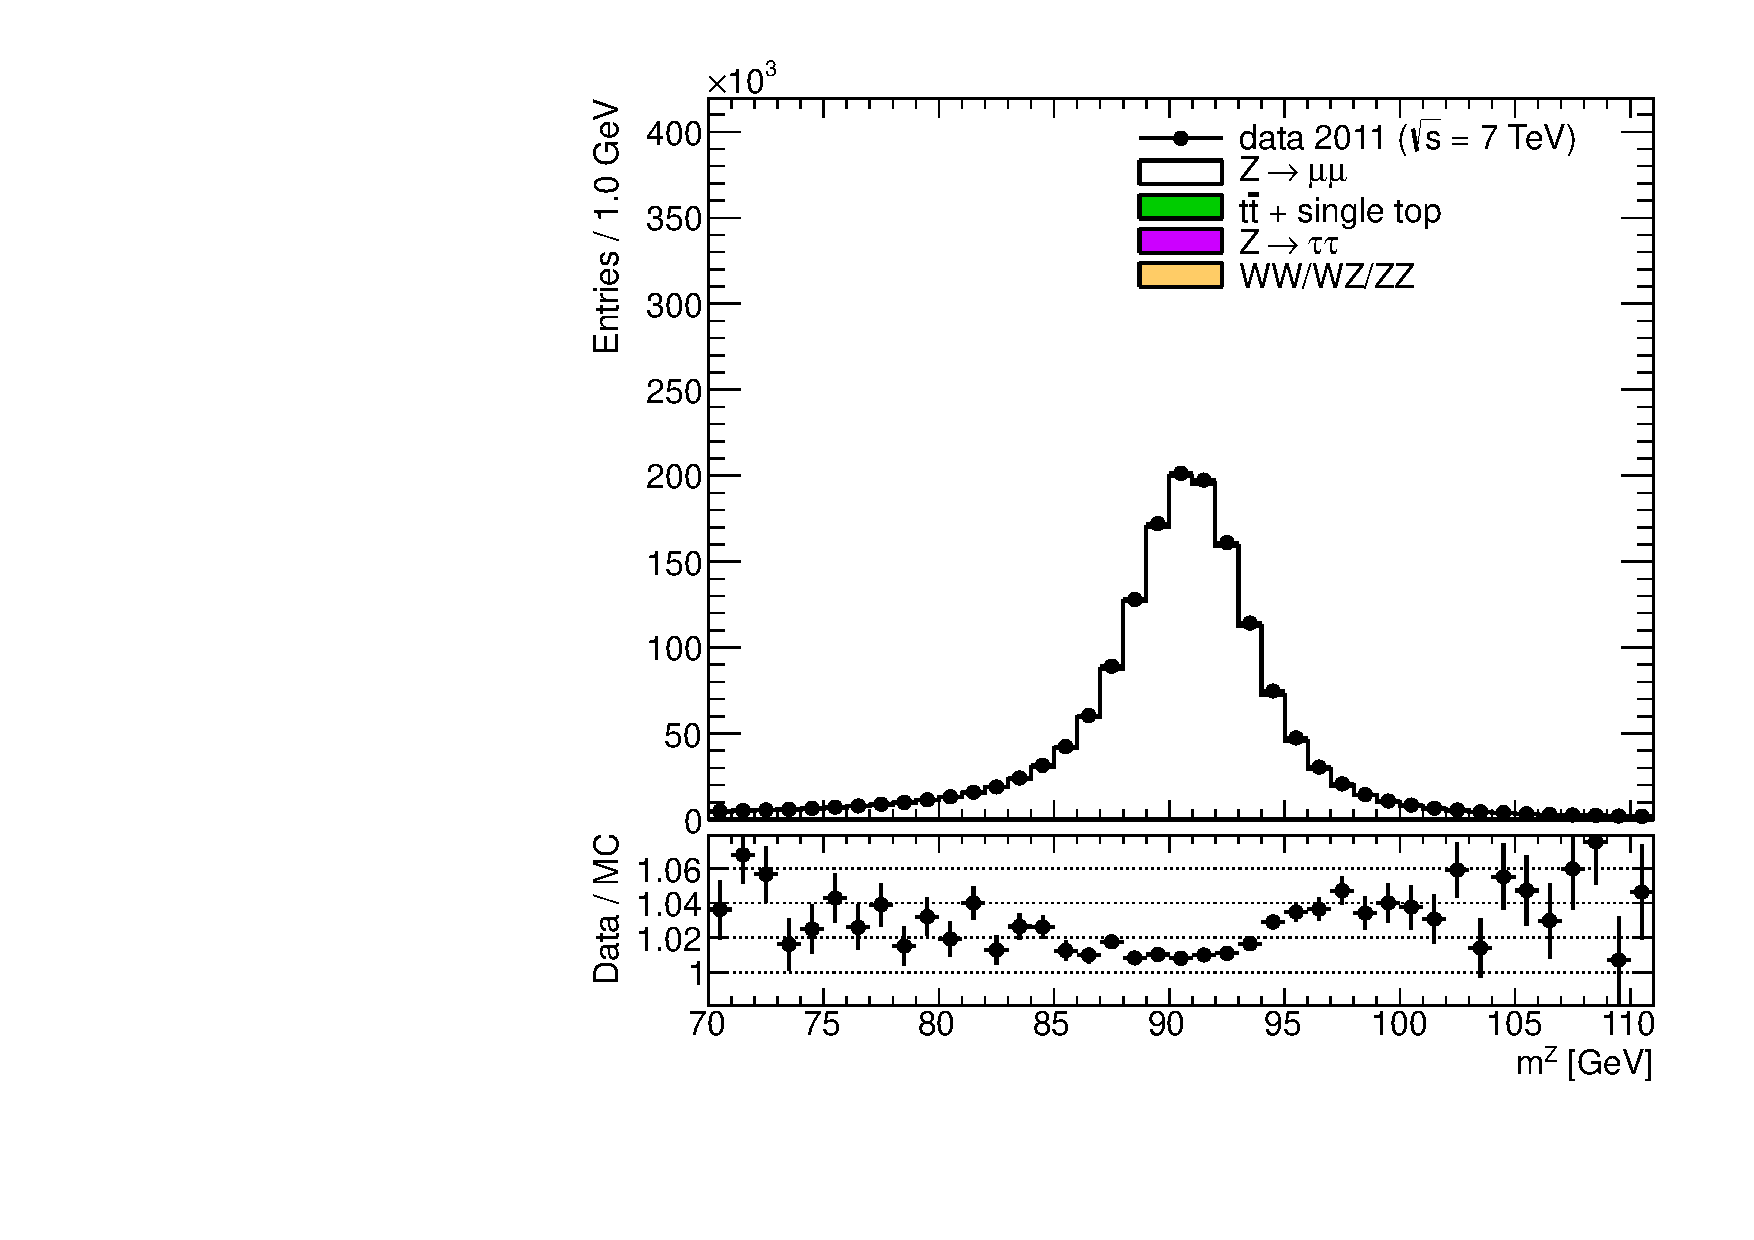
\includegraphics[height=0.9\textheight]{dates/20121119/figures/zplots/zm_nomatch.pdf}
}
